\documentclass[10pt]{beamer}
\usepackage[latin1]{inputenc}
\usepackage{amsmath}
\usepackage{amsfonts}
\usepackage{amssymb}
\usepackage{makeidx}
\usepackage{graphicx}
\usetheme{Antibes}
\usepackage{tikz}
%%%<
%\usepackage{verbatim}
%\usepackage[active,tightpage]{preview}
%\PreviewEnvironment{center}
%\setlength\PreviewBorder{10pt}%
%%%%>
\usetikzlibrary{arrows}

% Defines a `datastore' shape for use in DFDs.  This inherits from a
% rectangle and only draws two horizontal lines.
\makeatletter
\pgfdeclareshape{datastore}{
  \inheritsavedanchors[from=rectangle]
  \inheritanchorborder[from=rectangle]
  \inheritanchor[from=rectangle]{center}
  \inheritanchor[from=rectangle]{base}
  \inheritanchor[from=rectangle]{north}
  \inheritanchor[from=rectangle]{north east}
  \inheritanchor[from=rectangle]{east}
  \inheritanchor[from=rectangle]{south east}
  \inheritanchor[from=rectangle]{south}
  \inheritanchor[from=rectangle]{south west}
  \inheritanchor[from=rectangle]{west}
  \inheritanchor[from=rectangle]{north west}
  \backgroundpath{
    %  store lower right in xa/ya and upper right in xb/yb
    \southwest \pgf@xa=\pgf@x \pgf@ya=\pgf@y
    \northeast \pgf@xb=\pgf@x \pgf@yb=\pgf@y
    \pgfpathmoveto{\pgfpoint{\pgf@xa}{\pgf@ya}}
    \pgfpathlineto{\pgfpoint{\pgf@xb}{\pgf@ya}}
    \pgfpathmoveto{\pgfpoint{\pgf@xa}{\pgf@yb}}
    \pgfpathlineto{\pgfpoint{\pgf@xb}{\pgf@yb}}
 }
}
\makeatother


\title[Speaker recognition]{Machine Learning M2 project:\\
 Speaker recognition}
\author{Antoine Plet\\
Thomas Sibut-Pinote}
\institute{ENS de Lyon}
\logo{
\includegraphics[height=5mm]{logo.png}}

\begin{document}
\begin{frame}
\maketitle
\end{frame}


\begin{frame}


\begin{figure}[scale=0.1]
\centering
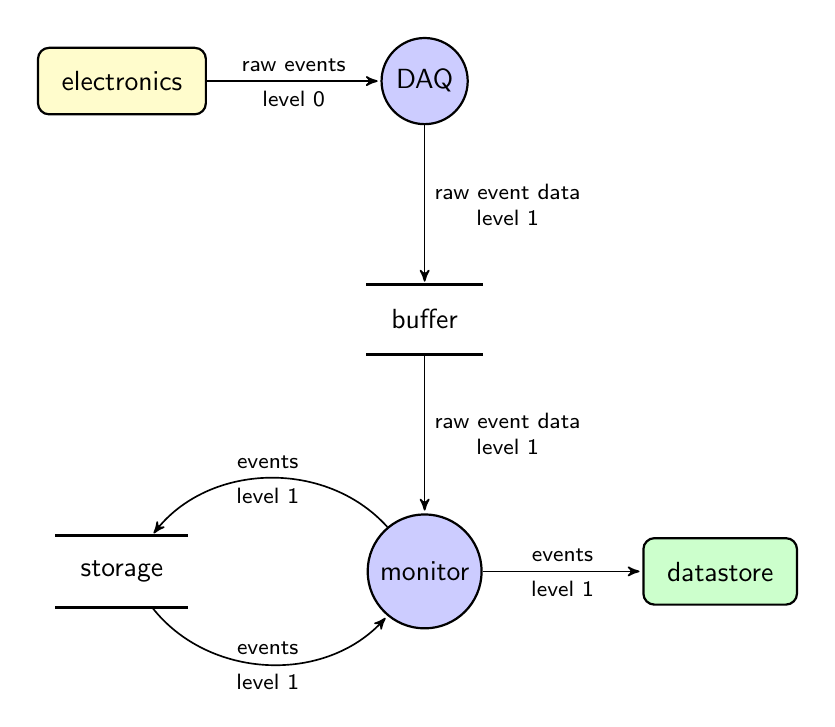
\begin{tikzpicture}[
  font=\sffamily,
  every matrix/.style={ampersand replacement=\&,column sep=2cm,row sep=2cm},
  source/.style={draw,thick,rounded corners,fill=yellow!20,inner sep=.3cm},
  process/.style={draw,thick,circle,fill=blue!20},
  sink/.style={source,fill=green!20},
  datastore/.style={draw,very thick,shape=datastore,inner sep=.3cm},
  dots/.style={gray,scale=2},
  to/.style={->,>=stealth',shorten >=1pt,semithick,font=\sffamily\footnotesize},
  every node/.style={align=center}]

  % Position the nodes using a matrix layout
  \matrix{
    \node[source] (hisparcbox) {electronics};
      \& \node[process] (daq) {DAQ}; \& \\

    \& \node[datastore] (buffer) {buffer}; \& \\

    \node[datastore] (storage) {storage};
      \& \node[process] (monitor) {monitor};
      \& \node[sink] (datastore) {datastore}; \\
  };

  % Draw the arrows between the nodes and label them.
  \draw[to] (hisparcbox) -- node[midway,above] {raw events}
      node[midway,below] {level 0} (daq);
  \draw[to] (daq) -- node[midway,right] {raw event data\\level 1} (buffer);
  \draw[to] (buffer) --
      node[midway,right] {raw event data\\level 1} (monitor);
  \draw[to] (monitor) to[bend right=50] node[midway,above] {events}
      node[midway,below] {level 1} (storage);
  \draw[to] (storage) to[bend right=50] node[midway,above] {events}
      node[midway,below] {level 1} (monitor);
  \draw[to] (monitor) -- node[midway,above] {events}
      node[midway,below] {level 1} (datastore);
\end{tikzpicture}
\end{figure}
\end{frame}

\begin{frame}{Data and preprocessing}
contenu...
\end{frame}

\begin{frame}{Stochastic gradient descent: optimization}
  $f_{obj}(w) := \frac{1}{2} \|w\|^2 + C\displaystyle\sum\limits_{i=1}^{n}l_i(w)$ with $l_i(w) := \mathrm{hinge}(y_i (w \cdot x_i + b))$
\begin{figure}[!h]
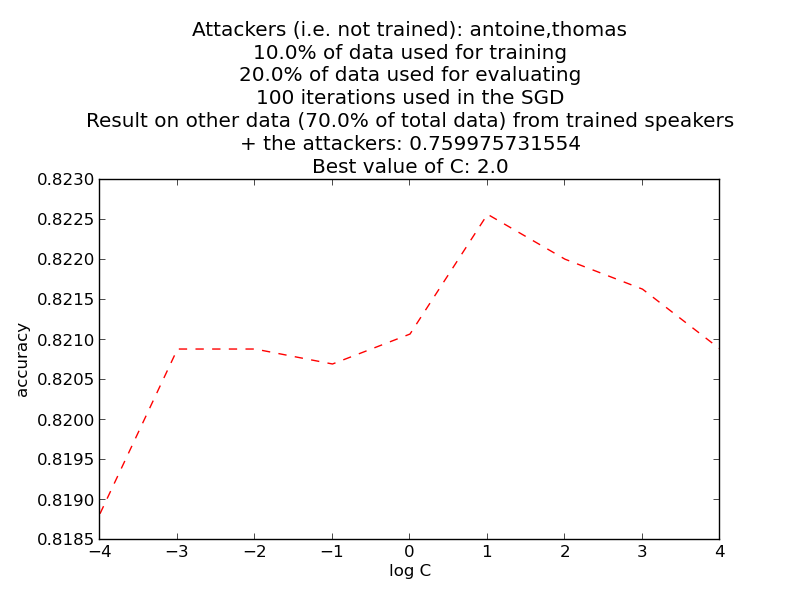
\includegraphics[width=0.5\textwidth]{../bestC}
\end{figure}
\end{frame}

\begin{frame}{Stochastic gradient descent: evaluation}
contenu...
\end{frame}

\begin{frame}{Fisher kernel}
contenu...
\end{frame}

\begin{frame}{Kernel perceptron: optimization}
We first used the Fisher kernel with the kernel perceptron algorithm.
%\begin{figure}[!h]
%\includegraphics[width=0.85\textwidth]{}
%\caption{Variation de la pr�cision en fonction du nombre de gausiennes}\label{opt_kp}
%\end{figure}

\end{frame}

\begin{frame}{Kernel perceptron: evaluation}
contenu...
\end{frame}

\begin{frame}{Quadratic optimization: optimization}
We then used a quadratic optimization with matlab to implement a new classifier.

\begin{figure}[!h]
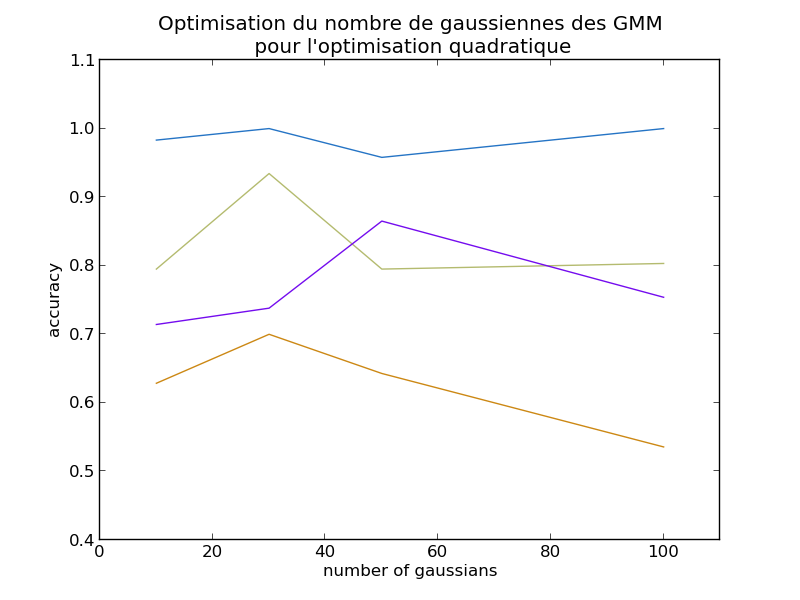
\includegraphics[width=0.5\textwidth]{../rapport/img/opt_qp_pdf}
\caption{Variation de la pr�cision en fonction du nombre de gausiennes}\label{opt_qp}
\end{figure}

\end{frame}

\begin{frame}{Quadratic optimization: evaluation}
contenu...
\end{frame}

\begin{frame}{Final exams}

\end{frame}

\begin{frame}{Conclusion}
  \begin{itemize}
    \item We implemented various classifiers based on SVM and compared them with one another
    \item
  \end{itemize}
\end{frame}

\begin{frame}
\fontsize{15}{17}\selectfont
\begin{center}
Thank you for your attention. \\
\vspace{.4in}
Any question?
\end{center}
\end{frame}

\end{document}